% -*- LaTeX -*-
% -*- coding: utf-8 -*-
%
% michael a.g. aïvázis <michael.aivazis@para-sim.com>
% (c) 2003-2017 all rights reserved
%

\section{applications}

% --------------------------------------
\subsection{simple}
\begin{frame}[fragile]
  \label{frame:applications-simple}
%
  \frametitle{A simple application script}
%
  \vskip -3ex
  \begin{itemize}
%
  \item \component{Stitcher}, a simple \pyrebuiltin{isce.application}
%
    \python{}{listings/stitch.py}
%
  \end{itemize}
%
\end{frame}

% --------------------------------------
\begin{frame}
%
  \frametitle{Applications as component containers}
%
  \vskip -3ex
  \begin{itemize}
%
  \item in \lstlineref{applications-simple-decl}, \component{Stitcher} derives from
    \pyrebuiltin{isce.application}
    \begin{itemize}
    \item which makes it a component
    \item with some special capabilities
    \item see \frameref{applications-plexus-pedigree} for its pedigree
    \end{itemize}
%
  \item in \lstlineref{applications-simple-dem}, \component{Stitcher} registers a requirement
    for a \protocol{dem} compatible implementation
    \begin{itemize}
    \item note the use of the protocol as the type of the trait
    \item the syntax is the same as for properties
    \item no explicit default is provided, so the protocol will be asked to provide one in the
      event that the user does not express a preference
    \end{itemize}
%
  \item the special behavior \method{main} in \lstlineref{applications-simple-main} is the
    application entry point
    \begin{itemize}
    \item it is invoked by the framework after the application instance is configured
    \end{itemize}
%
  \item the stanza after \lstlineref{applications-simple-boot} bootstraps the application:
    \begin{itemize}
    \item an instance is created and named
    \item the framework searches for a configuration file named after the instance
    \item the app is launched by invoking the method \method{run}
    \item the framework determines the hosting strategy based on the user's choice of
      application shell; the full details are on \frameref{applications-plexus-pedigree}
    \item it invokes the method \method{main} and collects the return status
    \item the status is shared with the user's environment by asking python to terminate in a
      controlled way
    \end{itemize}
%
  \end{itemize}
%
\end{frame}

% --------------------------------------
\subsection{configuration}
\begin{frame}
%
  \frametitle{Exercising the default configuration}
%
  \vskip -3ex
  \begin{itemize}
%
  \item let's focus on the relationship between \instance{stitch} and its trait \trait{dem}
%
  \item by the time we invoke the method \method{stitch} on
    \lstlineref{applications-simple-stitch}, we expect a fully configured instance of some
    component compatible with \protocol{isce.topography.dem}
%
  \item compatibility with the protocol guarantees that
    \begin{itemize}
    \item we have a way of specifying the region of interest
    \item the method \method{stitch} exists
    \end{itemize}
    since both of these are \protocol{isce.topography.dem} requirements
%
  \item if we provide no configuration
    \begin{itemize}
    \item evaluation of \literal{self.dem} will initiate a search for a suitable candidate
    \item the protocol will be asked to provide a default value, which will return the class
      record of \component{SRTM}
    \item since \component{SRTM} is assignment compatible with \protocol{isce.topography.dem},
      the framework will accept it as a viable candidate and configure it
    \item the framework will initiate the process of creating and configuring an instance with
      the name \literal{stitch.dem}, to match the name of the \component{Stitcher} property
    \item the instance will become the value of \literal{self.dem} for our application instance
    \item the method \method{stitch} will be invoked and find \trait{region} set to an empty
      \schema{array}, and \trait{resolution} set to \defaultvalue{1}
    \end{itemize}
%
  \item this is a typical strategy: by default, the app will function correctly but will not do
    much
%
  \end{itemize}
%
\end{frame}

% --------------------------------------
\begin{frame}
%
  \frametitle{The application inventory}
%
  \vskip -3ex
%
  here is a summary of what is and is not configurable with this particular implementation

  \begin{itemize}
  \item the \component{Stitcher} class declaration on \lstlineref{applications-simple-decl}
    does not specify a family name; \component{Stitcher} is not a public class, and there is
    no way to alter the settings for the class-wide defaults
  \item our application instance was given a name in the bootstrapping stanza after
    \lstlineref{applications-simple-boot}, so its \trait{dem} is under our control; it is
    accessible as \trait{stitch.dem}
  \item the \component{SRTM} class declaration has a family, so we can control the default
    values for \trait{region} and \trait{resolution} for all its instances; their names are
    \begin{itemize}
    \item \trait{isce.topography.dem.srtm.region}
    \item \trait{isce.topography.dem.srtm.resolution}
    \end{itemize}
    respectively (see \frameref{components-public})
  \item the \component{SRTM} instance that is bound to our application instance is accessible
    as \trait{stitch.dem}; hence its \trait{region} and \trait{resolution} values are
    accessible as
    \begin{itemize}
    \item \trait{stitch.dem.region}
    \item \trait{stitch.dem.resolution}
    \end{itemize}
    respectively (again, see \frameref{components-public})
  \end{itemize}

\end{frame}

% --------------------------------------
\begin{frame}[fragile]
%
  \frametitle{Configuration from the command line}
%
  \vskip -3ex
  \begin{itemize}
%
  \item suppose that the code on \frameref{applications-simple} is in a script called
    \package{stitch.py}; we don't have an alternative implementation of
    \protocol{isce.topography.dem}, but we can be explicit about the one we have
    \begin{ish}[gobble=4, numbers=none]{}
      ~/tmp> stitch.py --stitch.dem=isce.topography.dem.srtm
    \end{ish}
%
  \item application traits are automatically available at the top level of the namespace, so we
    can shorten this to
    \begin{ish}[gobble=4, numbers=none]{}
      ~/tmp> stitch.py --dem=isce.topography.dem.srtm
    \end{ish}
%
  \item we can take advantage of the rational organization of the \isce\ namespace to
    shorten this further
    \begin{ish}[gobble=4, numbers=none]{}
      ~/tmp> stitch.py --dem=srtm
    \end{ish}
%
\item we can also control any property of \trait{dem}
    \begin{ish}[gobble=4, numbers=none]{}
      ~/tmp> stitch.py --dem=srtm --dem.resolution=3
    \end{ish}
%
  \item mistakes are flagged
    \begin{ish}[gobble=4, numbers=none]{}
      ~/tmp> stitch.py --dem=madeup
      stitch: could not resolve 'madeup' into a component that implements
      protocol 'isce.topography.dem'
    \end{ish}
%
  \item the right hand side of the \trait{dem} assignment has a very rich syntax and is a
    critical part of the extensibility of our applications
%
  \end{itemize}
%
\end{frame}

% --------------------------------------
\begin{frame}[fragile]
%
  \label{frame:applications-config}
%
  \frametitle{Application configuration files}
%
  \vskip -3ex
  \begin{itemize}
%
  \item settings that we expect to change less frequently can be placed in configuration files;
    let's adapt the sample from \frameref{srtm-pfg}
%
    \pfg{firstnumber=7, linerange={7-20}}{listings/stitch.pfg}
%
  \item the ability to capture the namespace hierarchy with the block structure makes for very
    readable configuration files
%
  \item the simplicity of the syntax helps as well
%
  \item there are many ways to force the framework to recognize these settings
    \begin{itemize}
    \item the natural one is to place them in a file called \package{stitch.pfg} in the working
      directory
    \item see \frameref{applications-config-sources} for a more complete picture
    \end{itemize}
%
  \end{itemize}
%
\end{frame}

% --------------------------------------
\begin{frame}
%
  \label{frame:applications-config-conditional}
%
  \frametitle{Conditional assignments}
%
  \vskip -3ex
  \begin{itemize}
%
  \item the settings on \frameref{applications-config} contain a subtle bug:
    \begin{itemize}
    \item setting \trait{region} is ok, since the \protocol{isce.topography.dem} forces all
      compatible implementations to have this trait
    \item but this is not the case with \trait{resolution}
    \end{itemize}
%
  \item an option is to set a default resolution for all instances of \component{SRTM}, but in
    general this is not the right solution; besides, it only works if every use of
    \component{SRTM} requires the high resolution tiles
%
  \item what we need is a way to express the following: if \trait{stitch.dem} is an instance of
    \component{isce.topography.dem.srtm}, then set \trait{resolution} to 1
%
  \item there is special syntax for this use case; see
    \lstlineref{applications-conditional-syntax} below
%
    \pfg{firstnumber=7, linerange={7-18}}{listings/stitch-conditional.pfg}
%
  \item now the setting applies only when \trait{dem} is bound to an \component{SRTM} instance
%
  \end{itemize}
%
\end{frame}

% --------------------------------------
\begin{frame}
%
  \frametitle{Configuration event ranking}
%
  \vskip -3ex
  \begin{itemize}
%
  \item each configuration event is assigned a priority when it is encountered
    \begin{itemize}
    \item the priority is a pair: (category, collation sequence)
    \item the priority category is determined by the event source
    \item whether and event has an effect on the corresponding trait depends on the priority of
      the current value
    \item this way the framework can respond correctly to newly discovered information
    \end{itemize}
%
  \item the framework recognizes the following priority categories, in increasing order
%
    \begin{itemize}
%
    \item defaults: values from component trait declarations in the source code
      \begin{itemize}
      \item this is the developer's contribution
      \end{itemize}
%
    \item boot: assigned while the framework is booting
      \begin{itemize}
      \item currently, assigned to the values of user environment variables
      \end{itemize}
%
    \item package: values from configuration files in the install directory of a package
      \begin{itemize}
      \item this is the sysadmin's opportunity to configure a package for users on a given
        system
      \end{itemize}
%
    \item user: values from the user's configuration files, typically in \url{~/.pyre}
      \begin{itemize}
      \item this is the user's opportunity to override package settings
      \end{itemize}
%
    \item command line: the priority of values retrieved from the command line for the current
      invocation of the application
%
    \item explicit: direct assignments in user code
      \begin{itemize}
      \item in general, this is discouraged unless configuring a subcomponent
      \end{itemize}
%
    \item framework: a priority that essentially renders values as read-only
%
    \end{itemize}
%
  \end{itemize}
%
\end{frame}

% --------------------------------------
\begin{frame}
%
  \label{frame:applications-config-sources}
%
  \frametitle{Configuration event sources}
%
  \vskip -3ex
  \begin{itemize}
%
  \item configuration is a dynamic process in \pyre; it happens both explicitly, such as
    when processing the command line arguments, and implicitly, when encountering a new package
%
    \begin{itemize}
    \item compliant packages register themselves with the framework
    \item the framework forms a filename out of the package name and an extension from each
      register configuration codec
    \item a search over the locations on the \trait{configpath} is initiated
    \item all matching configuration files are loaded
    \end{itemize}
%
  \item by default, \trait{configpath} knows about the \pyre\ install location, the user's
    \url{.pyre} directory, and the current working directory
%
  \item this process cascades into the dependencies of each package
    \begin{itemize}
    \item for example, on \lstlineref{applications-simple-import} of
      \frameref{applications-simple}, we \keyword{import} \isce\, which in turn imports \pyre
    \item this means that a search for \literal{pyre.\{pfg,cfg,pml\}} is initiated, and every
      match is loaded
    \item followed by a search for \literal{isce.\{pfg,cfg,pml\}}
    \end{itemize}
%
  \item similarly, while building the application instance, the framework conducts a search for
    a configuration file derived out of the instance name, and loads any matches
    \begin{itemize}
    \item this is the preferred way to configure an application implicitly; the others are
      meant to modify the defaults from the source code
    \end{itemize}
%
  \item while processing the command line arguments
%
  \item by invoking the application with an \literal{-{}-config} argument
%
  \item in user code, by invoking the function \function{loadConfiguration()} explicitly
%
  \end{itemize}
%
\end{frame}

% --------------------------------------
\subsection{integration}
\begin{frame}[fragile]
%
  \label{frame:applications-help}
%
  \frametitle{Providing help}
%
  \vskip -3ex
  \begin{itemize}
%
  \item components that derive from \component{isce.application} have another behavior,
    \method{help}
    \begin{itemize}
    \item it is tied to a family of command line arguments:
    \end{itemize}
%
  \item the default implementation displays a help screen
    \begin{ish}[gobble=4]{}
      ~/tmp> stitch.py --help
      stitch:

          Stitch together a DEM for some region

      usage:

          stitch [options]

      options:
            --dem: the assembler of the elevation model [component]
          --shell: my hosting strategy [component]
          --DEBUG: debugging mode [bool]

      ~/tmp>
    \end{ish}
%
  \item the default set is: \literal{-h}, \literal{-?} and \literal{-help}
    \begin{itemize}
    \item configurable, since it is a property of the application \component{shell}
    \end{itemize}
%
  \item the framework interrogates the application instance and generates this information
%
  \item applications can customize what is displayed by overriding the hook \method{pyre\_help},
    an application method that takes no additional arguments and returns a sequence of strings
%
  \end{itemize}
%
\end{frame}

% --------------------------------------
\begin{frame}
%
  \frametitle{Virtual filesystems}
%
  \begin{itemize}
%
  \item virtual, local, zip, hdf5
%
  \item apps
    \begin{itemize}
    \item vfs, pfs
    \item \method{pyre\_explore}, \method{pyre\_mountApplicationFolders}, \method{pyre\_mountPrivateFilespace},
      \method{pyre\_mountPrivateFolder}
    \item standard fs layout
    \end{itemize}
%
  \end{itemize}
%
\end{frame}

% --------------------------------------
\begin{frame}
%
  \frametitle{Framework services for applications}
%
  \begin{itemize}
  \item programming patterns (patterns)
  \item primitives: path, uri (primitives)
  \item evaluation networks (algebraic, calc)
  \item csg primitives (geometry)
  \item multidimensional arrays (grid)
  \item filesystems (filesystem)
  \item performance monitoring (timers)
  \item content generators (weaver)
  \item scanners and parsers (tracking, parsing, xml)
  \item external dependencies (platforms, externals)
  \item event driven and asynchronous apps (ipc, nexus, http)
  \item records, tables, and databases (db, records, tabular)
  \end{itemize}
%
\end{frame}

% --------------------------------------
\subsection{shells}
\begin{frame}
%
  \frametitle{The \component{script} shell}
%
  \begin{itemize}
%
  \item components that derive from \component{isce.application} have a property \trait{shell}
    \begin{itemize}
    \item we saw this on \frameref{applications-help}
    \end{itemize}
%
  \item the shell is the link between the call to \literal{app.run()} on
    \lstlineref{applications-simple-run} and the behavior \method{main} on
    \lstlineref{applications-simple-main} on \frameref{applications-simple}
    \begin{itemize}
    \item it helps us factor out how the application is invoked after it is configured
    \end{itemize}
%
  \item shells must implement the protocol \protocol{pyre.shells}; there are two requirements
    \begin{itemize}
    \item the trait \trait{home} is a \basictype{str} that gives the user control over the
      preferred working directory for the application
    \item the method \method{launch} is the staging strategy of the shell
    \end{itemize}
%
  \item the application method \method{run} simply invokes the method \method{launch} of its
    shell, and passes itself as an argument
%
  \item the protocol \protocol{pyre.shells} specifies \component{script} as the default shell
%
  \item the method \method{launch} of \component{script} is trivial: it just invokes \method{main}
    of whatever application object it receives as an argument
%
  \item any additional arguments to \method{run} are just carried through to \method{main}
%
  \end{itemize}
%
\end{frame}

% --------------------------------------
\begin{frame}[fragile]
%
  \frametitle{The \component{interactive} shell}
%
  \begin{itemize}
%
  \item occasionally, users find it useful to poke around applications interactively
%
    \begin{ish}[gobble=4]{}
      ~/tmp> stitch.py --shell=interactive
      stitch:

          Stitch together a DEM for some region

      usage:

          stitch [options]

      options:
            --dem: the assmebler of the elevation model [component]
          --shell: my hosting strategy [component]
          --DEBUG: debugging mode [bool]

      entering interactive mode...

      stitch: dir()
      ['__builtins__', 'app']
      stitch:
    \end{ish}
%
  \item users can now invoke application methods through the variable \instance{app}
%
  \item further, all framework services are now accessible interactively
    \begin{itemize}
    \item for example, the executive, a singleton\supercite{patterns} that serves as the anchor
      of all framework services, is accessible through \instance{app.pyre\_executive}
    \end{itemize}
%
  \end{itemize}
%
\end{frame}

% --------------------------------------
\begin{frame}[fragile]
%
  \frametitle{The \component{web} shell}
%
  \vskip -3ex
  \begin{itemize}
%
  \item a fairly recent addition is the shell \component{web}
%
    \begin{ish}[gobble=4]{}
      ~/tmp> stitch.py --shell=web
      stitch: web server on '0.0.0.0':62859
      ...
    \end{ish}
%
  \item \component{web}
    \begin{itemize}
    \item grabs a port on the local machine
    \item launches a web server that listens to this port for incoming connections
    \item launches a web browser with a url that points to this server
    \end{itemize}
%
  \item the default behavior is not very exciting currently (\pyre\ 1.0 revno 2787)

    \begin{center}
      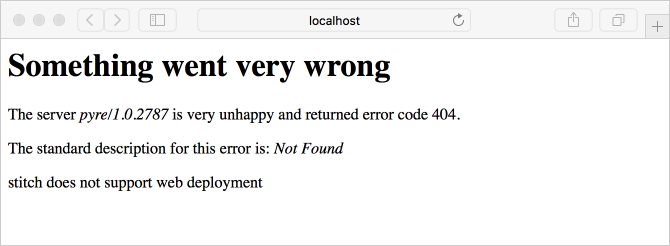
\includegraphics[width=0.5\textwidth]{stitcher-web}
    \end{center}
%
  \item the web server is a \pyre\ service, and under total application developer control
%
  \item this opens up the possibility of extremely powerful, portable, interactive applications
    \begin{itemize}
    \item currently a major thrust in \pyre\ development
    \end{itemize}
%
  \end{itemize}
%
\end{frame}

% --------------------------------------
\subsection{plexus}
\begin{frame}[fragile]
%
  \frametitle{Support for behavior rich applications}
%
  \vskip -3ex
  \begin{itemize}
%
  \item \component{stitch} is an example of a single purpose application
    \begin{itemize}
    \item its name describes what it does
    \item its behavior is encapsulated in its \method{main} behavior
    \end{itemize}
%
  \item with the command line as the user interface, more complex behavior can be encapsulated
    by using
    \begin{itemize}
    \item commands: words that invoke the named behavior
    \item panels: containers of commands
    \end{itemize}
%
  \item the UX design goal is memorable sentences
%
  \item the \isce\ application itself is an example; typical usage:
    \begin{ish}{}
      ~/tmp> isce srtm download --region='(33,-118), (35,-116)'
    \end{ish}
%
  \item this mimics the interaction with the menu structure of a graphical application
    \begin{itemize}
    \item however, the pattern is much older: your unix shell is the prototypical example...
    \end{itemize}
%
  \item the framework base class that enables this behavior is \component{isce.plexus}
    \begin{itemize}
    \item its \method{main} method is responsible for interpreting the first
      non-configurational command line argument as an \protocol{action} implementation
    \item its \method{help} introspects to build a list of known commands
    \end{itemize}
%
  \item behavior is provided in terms of components that implement the protocol
    \protocol{isce.action}, usually by deriving from
    \begin{itemize}
    \item \component{isce.command()} (see \frameref{applications-plexus-command})
    \item \component{isce.panel()} (see \frameref{applications-plexus-pannel})
    \end{itemize}
%
  \end{itemize}
%
\end{frame}

% --------------------------------------
\begin{frame}[fragile]
%
  \frametitle{The \isce\ default screen}
%
  \begin{itemize}
%
  \item launching \isce\ without any arguments generates the following:
%
    \begin{ish}[gobble=4]{}
      ~/tmp> isce
      isce:
          isce 3.0 revision 161
          copyright (c) 2003-2017 all rights reserved

      authors:
          Piyush Agram        <piyush.agram@jpl.nasa.gov>
          Michael Aivazis     <michael.aivazis@para-sim.com>
          Eric Gurrola        <eric.m.gurrola@jpl.nasa.gov>
          Paul Rosen          <paul.a.rosen@jpl.nasa.gov>
          Giangi Sacco        <gianfranco.sacco@jpl.nasa.gov>

      license:
          The complete usage terms can be found in the file LICENSE.txt

      commands:
            dem: download and assemble digital elevation models
           srtm: manage the local cache of the SRTM data store
          about: display information about this application
    \end{ish}
%
  \end{itemize}
%
\end{frame}

% --------------------------------------
\begin{frame}[fragile]
%
  \frametitle{Application introspection: the action \component{about}}
%
  \begin{itemize}
%
  \item the built-in action \component{about} displays information about the application
%
    \begin{ish}[gobble=4]{}
      ~/tmp> isce about
      isce: isce about

          Display information about this application

      usage:
          isce about [command]

      where [command] is one of
               name: the name of the app for configuration purposes
               home: the application home directory
             prefix: the application installation directory
           defaults: the application configuration directory
            version: print the version number
          copyright: print the copyright note
            credits: print out the acknowledgments
            license: print out the license and terms of use
                nfs: dump the application configuration namespace
                pfs: dump the application private filesystem
                vfs: dump the application virtual filesystem
               help: show this help screen

      options:
          --root: specify the portion of the namespace to display [str]
           --dry: show what would get done without actually doing anything [bool]
    \end{ish}
%
  \end{itemize}
%
\end{frame}

% --------------------------------------
\begin{frame}[fragile]
%
  \label{frame:applications-plexus-command}
%
  \frametitle{Extending the set of actions}
%
  \vskip -3ex
  \begin{itemize}
%
  \item end users can add actions to \isce\ very easily
%
  \item let's place the following code in \url{~/.pyre/isce/actions/say.py}
%
    \python{}{listings/say-command.py}
%
  \end{itemize}
 %
\end{frame}

% --------------------------------------
\begin{frame}[fragile]
%
  \frametitle{Extending the set of actions}
%
  \vskip -3ex
  \begin{itemize}
%
  \item with the user action installed, the \isce\ main help screen includes the new action
    \component{say}
%
    \begin{ish}[gobble=4]{}
      ~/tmp> isce
      isce:
          isce 3.0 revision 161
          copyright (c) 2003-2017 all rights reserved

      authors:
          Piyush Agram        <piyush.agram@jpl.nasa.gov>
          Michael Aivazis     <michael.aivazis@para-sim.com>
          Eric Gurrola        <eric.m.gurrola@jpl.nasa.gov>
          Paul Rosen          <paul.a.rosen@jpl.nasa.gov>
          Giangi Sacco        <gianfranco.sacco@jpl.nasa.gov>

      license:
          The complete usage terms can be found in the file LICENSE.txt

      commands:
            say: an example of a custom action provided by the end user
            dem: download and assemble digital elevation models
           srtm: manage the local cache of the SRTM data store
          about: display information about this application
    \end{ish}
%
  \item invoking it yields
%
    \begin{ish}{}
      ~/tmp> isce say
      isce: hello world!
    \end{ish}
%
  \end{itemize}
%
\end{frame}

% --------------------------------------
\begin{frame}[fragile]
%
  \label{frame:applications-plexus-pannel}
%
  \frametitle{Creating a new \isce\ panel}
%
  \begin{itemize}
%
  \item we can turn the new command into a panel by changing a few lines of code
%
    \python{}{listings/say-panel.py}
%
  \end{itemize}
%
\end{frame}

% --------------------------------------
\begin{frame}[fragile]
%
  \frametitle{Invoking the panel extension}
%
  \begin{itemize}
%
  \item invoking it now produces
%
    \begin{ish}[gobble=4]{}
      ~/tmp> isce say
      isce: isce say

          An example of a custom action provided by the end user

      usage:
          isce say [command]

      where [command] is one of
         hello: an example of a custom behavior
          help: show this help screen

      options:
          --dry: show what would get done without actually doing anything [bool]

      ~/tmp>
    \end{ish}
%
  \item we can invoke \method{hello} to get
%
    \begin{ish}[firstnumber=16, gobble=4]{}
      ~/tmp> isce say hello
      isce: hello world!
    \end{ish}
%
  \end{itemize}
%
\end{frame}

% --------------------------------------
\begin{frame}
%
  \label<6>{frame:applications-plexus-pedigree}
%
  \frametitle{The \component{isce.plexus} structure}
%
  \vskip -3ex
  \only<1>{
    \begin{center}
      
\includegraphics[width=0.9\textwidth]{pyre-plexus-base}
    \end{center}
  }
  \only<2>{
    \begin{center}
      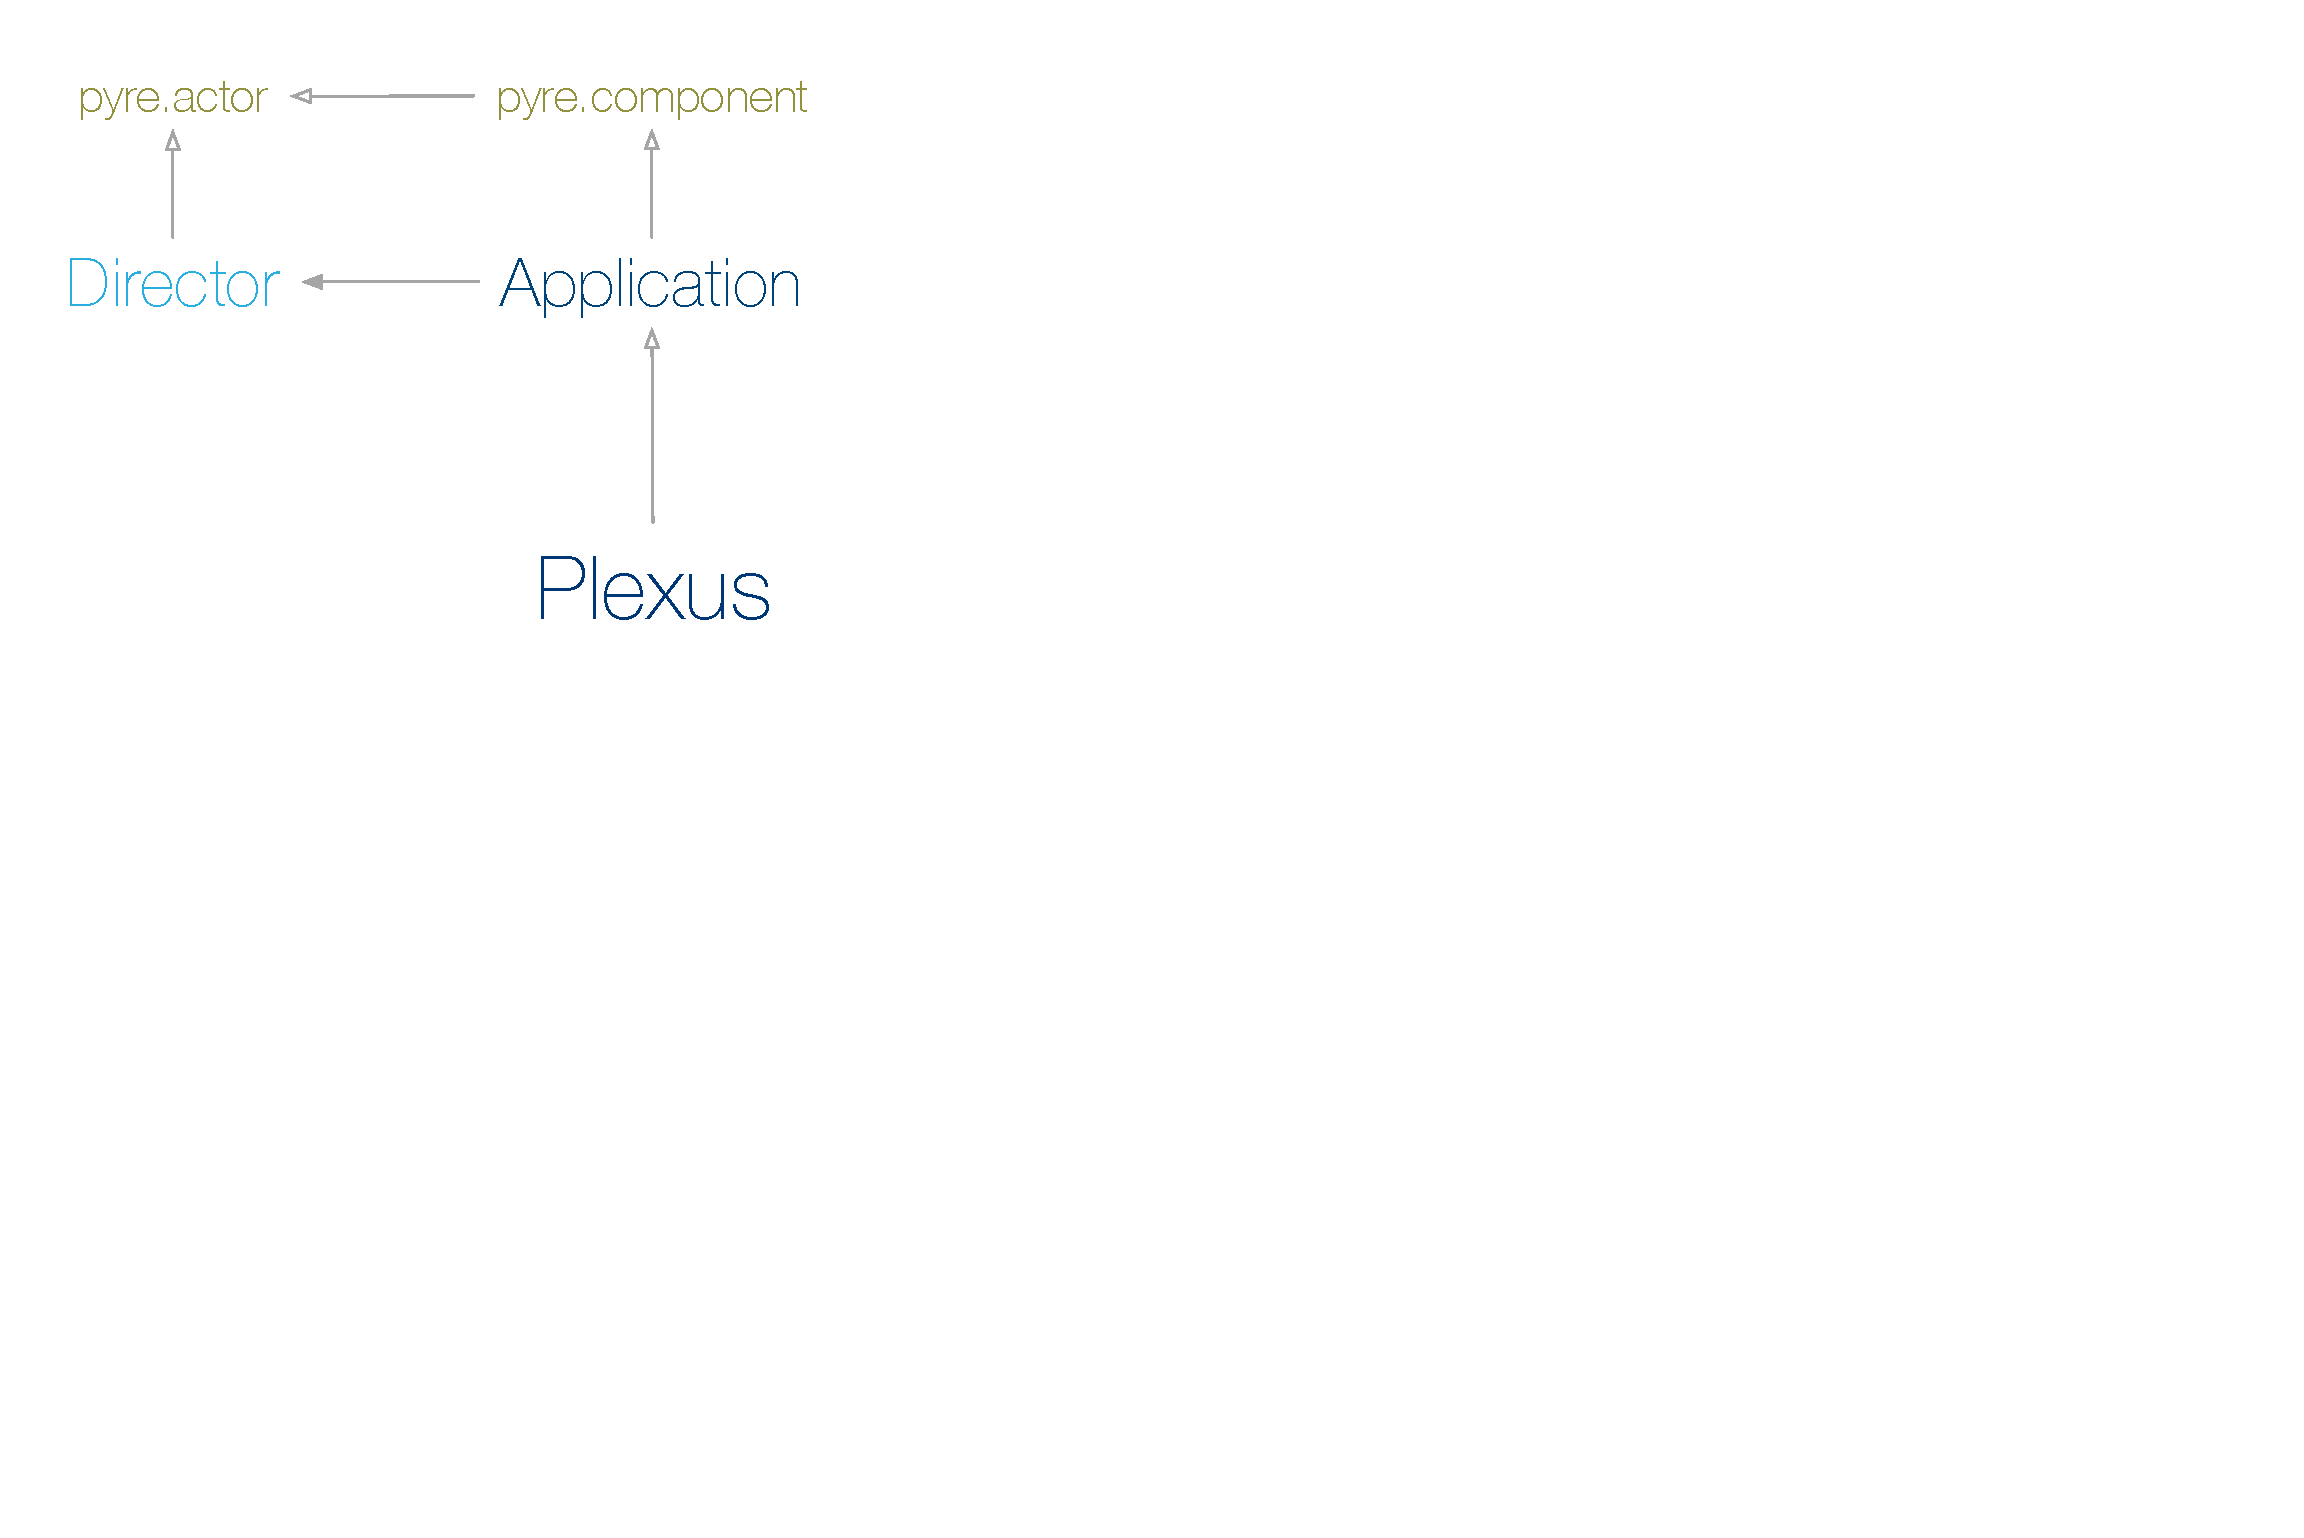
\includegraphics[width=0.9\textwidth]{pyre-plexus-pedigree}
    \end{center}
  }
  \only<3>{
    \begin{center}
      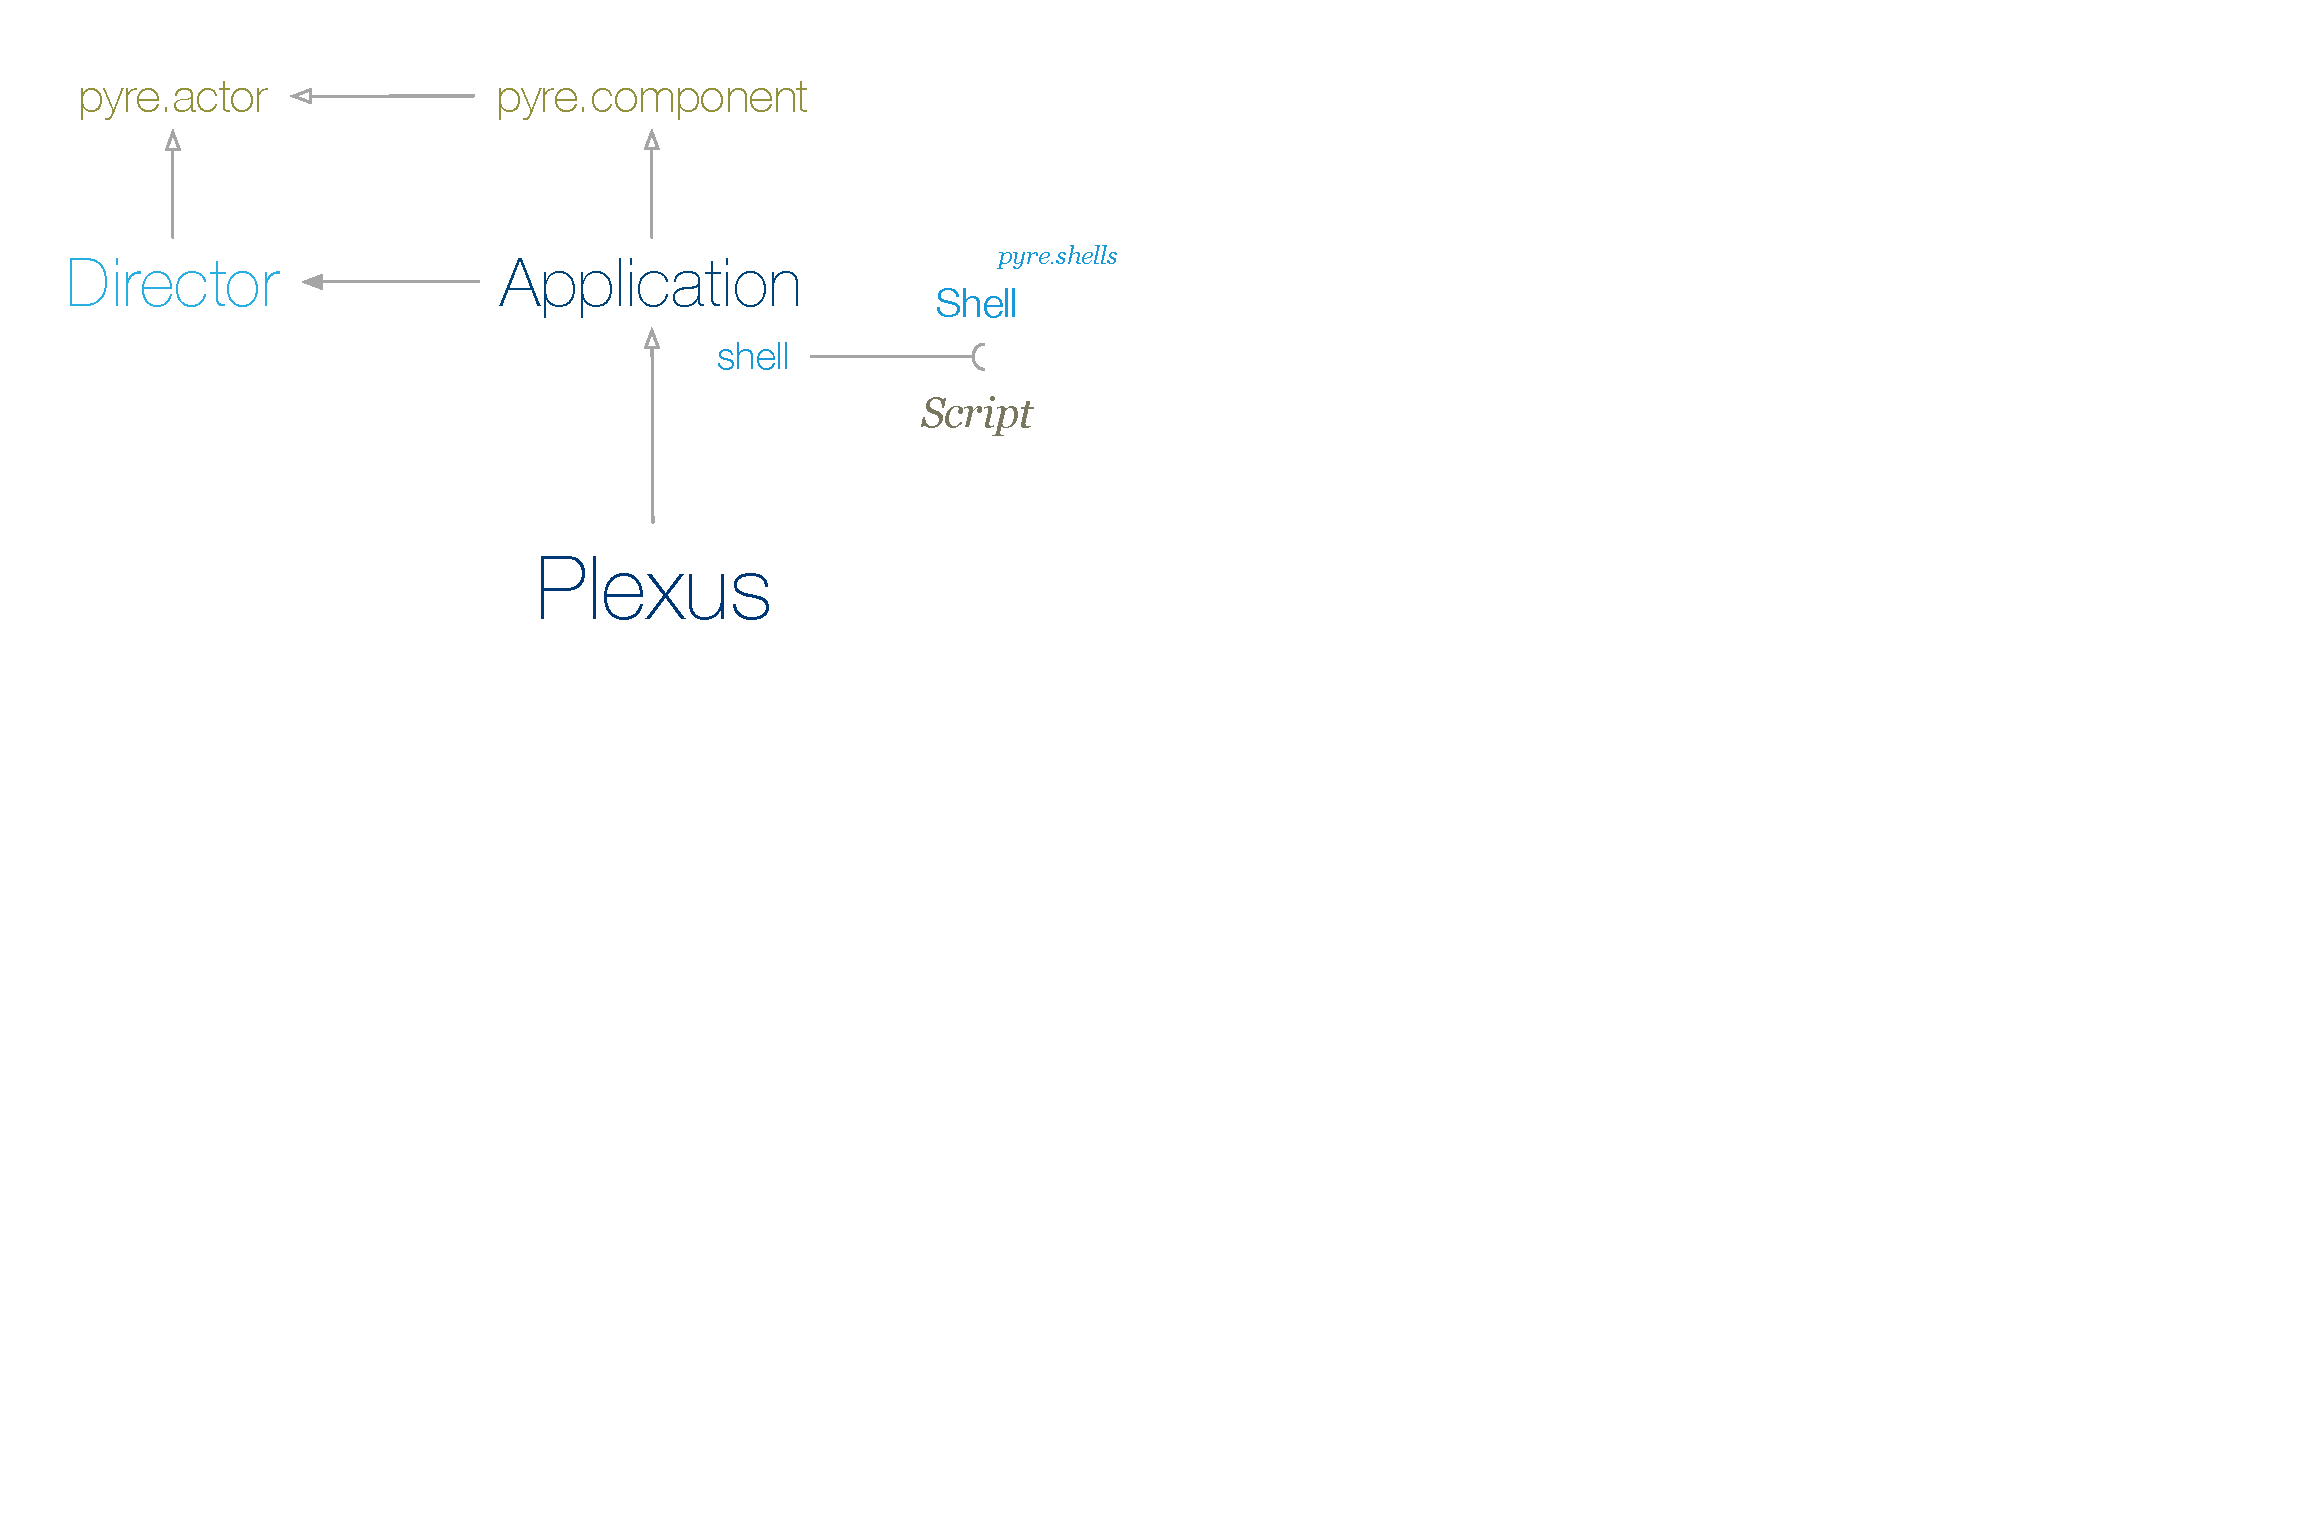
\includegraphics[width=0.9\textwidth]{pyre-plexus-traits}
    \end{center}
  }
  \only<4>{
    \begin{center}
      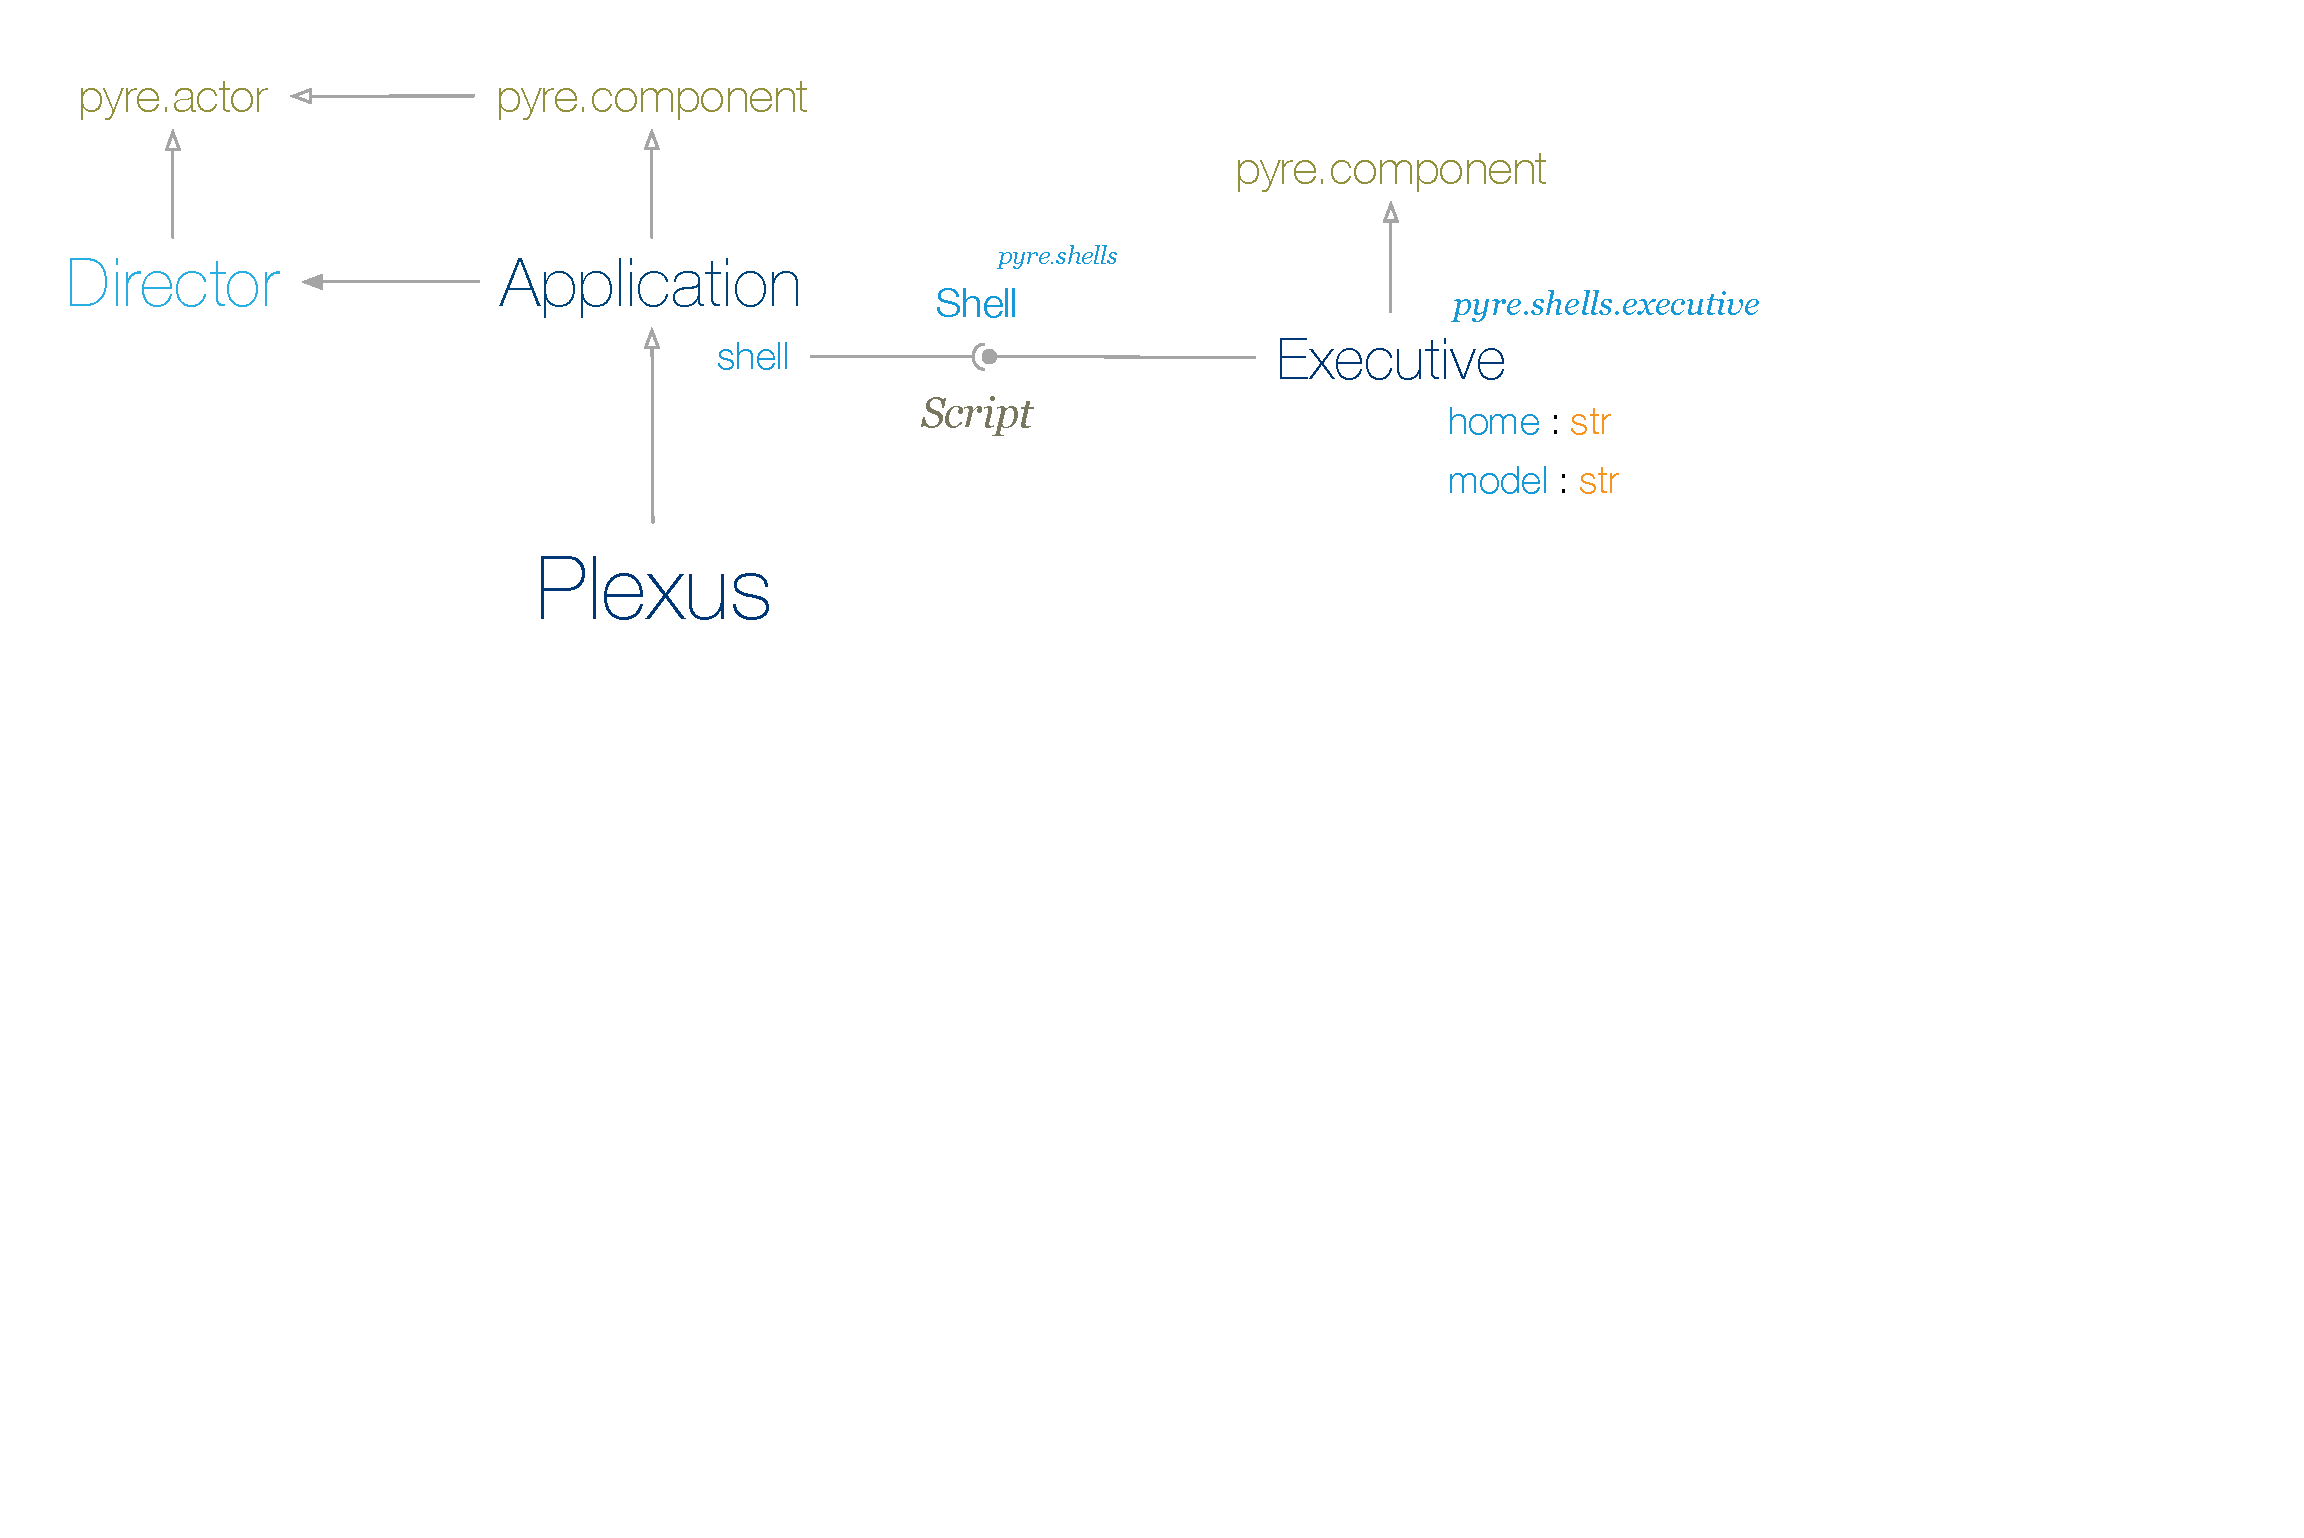
\includegraphics[width=0.9\textwidth]{pyre-plexus-executive}
    \end{center}
  }
  \only<5>{
    \begin{center}
      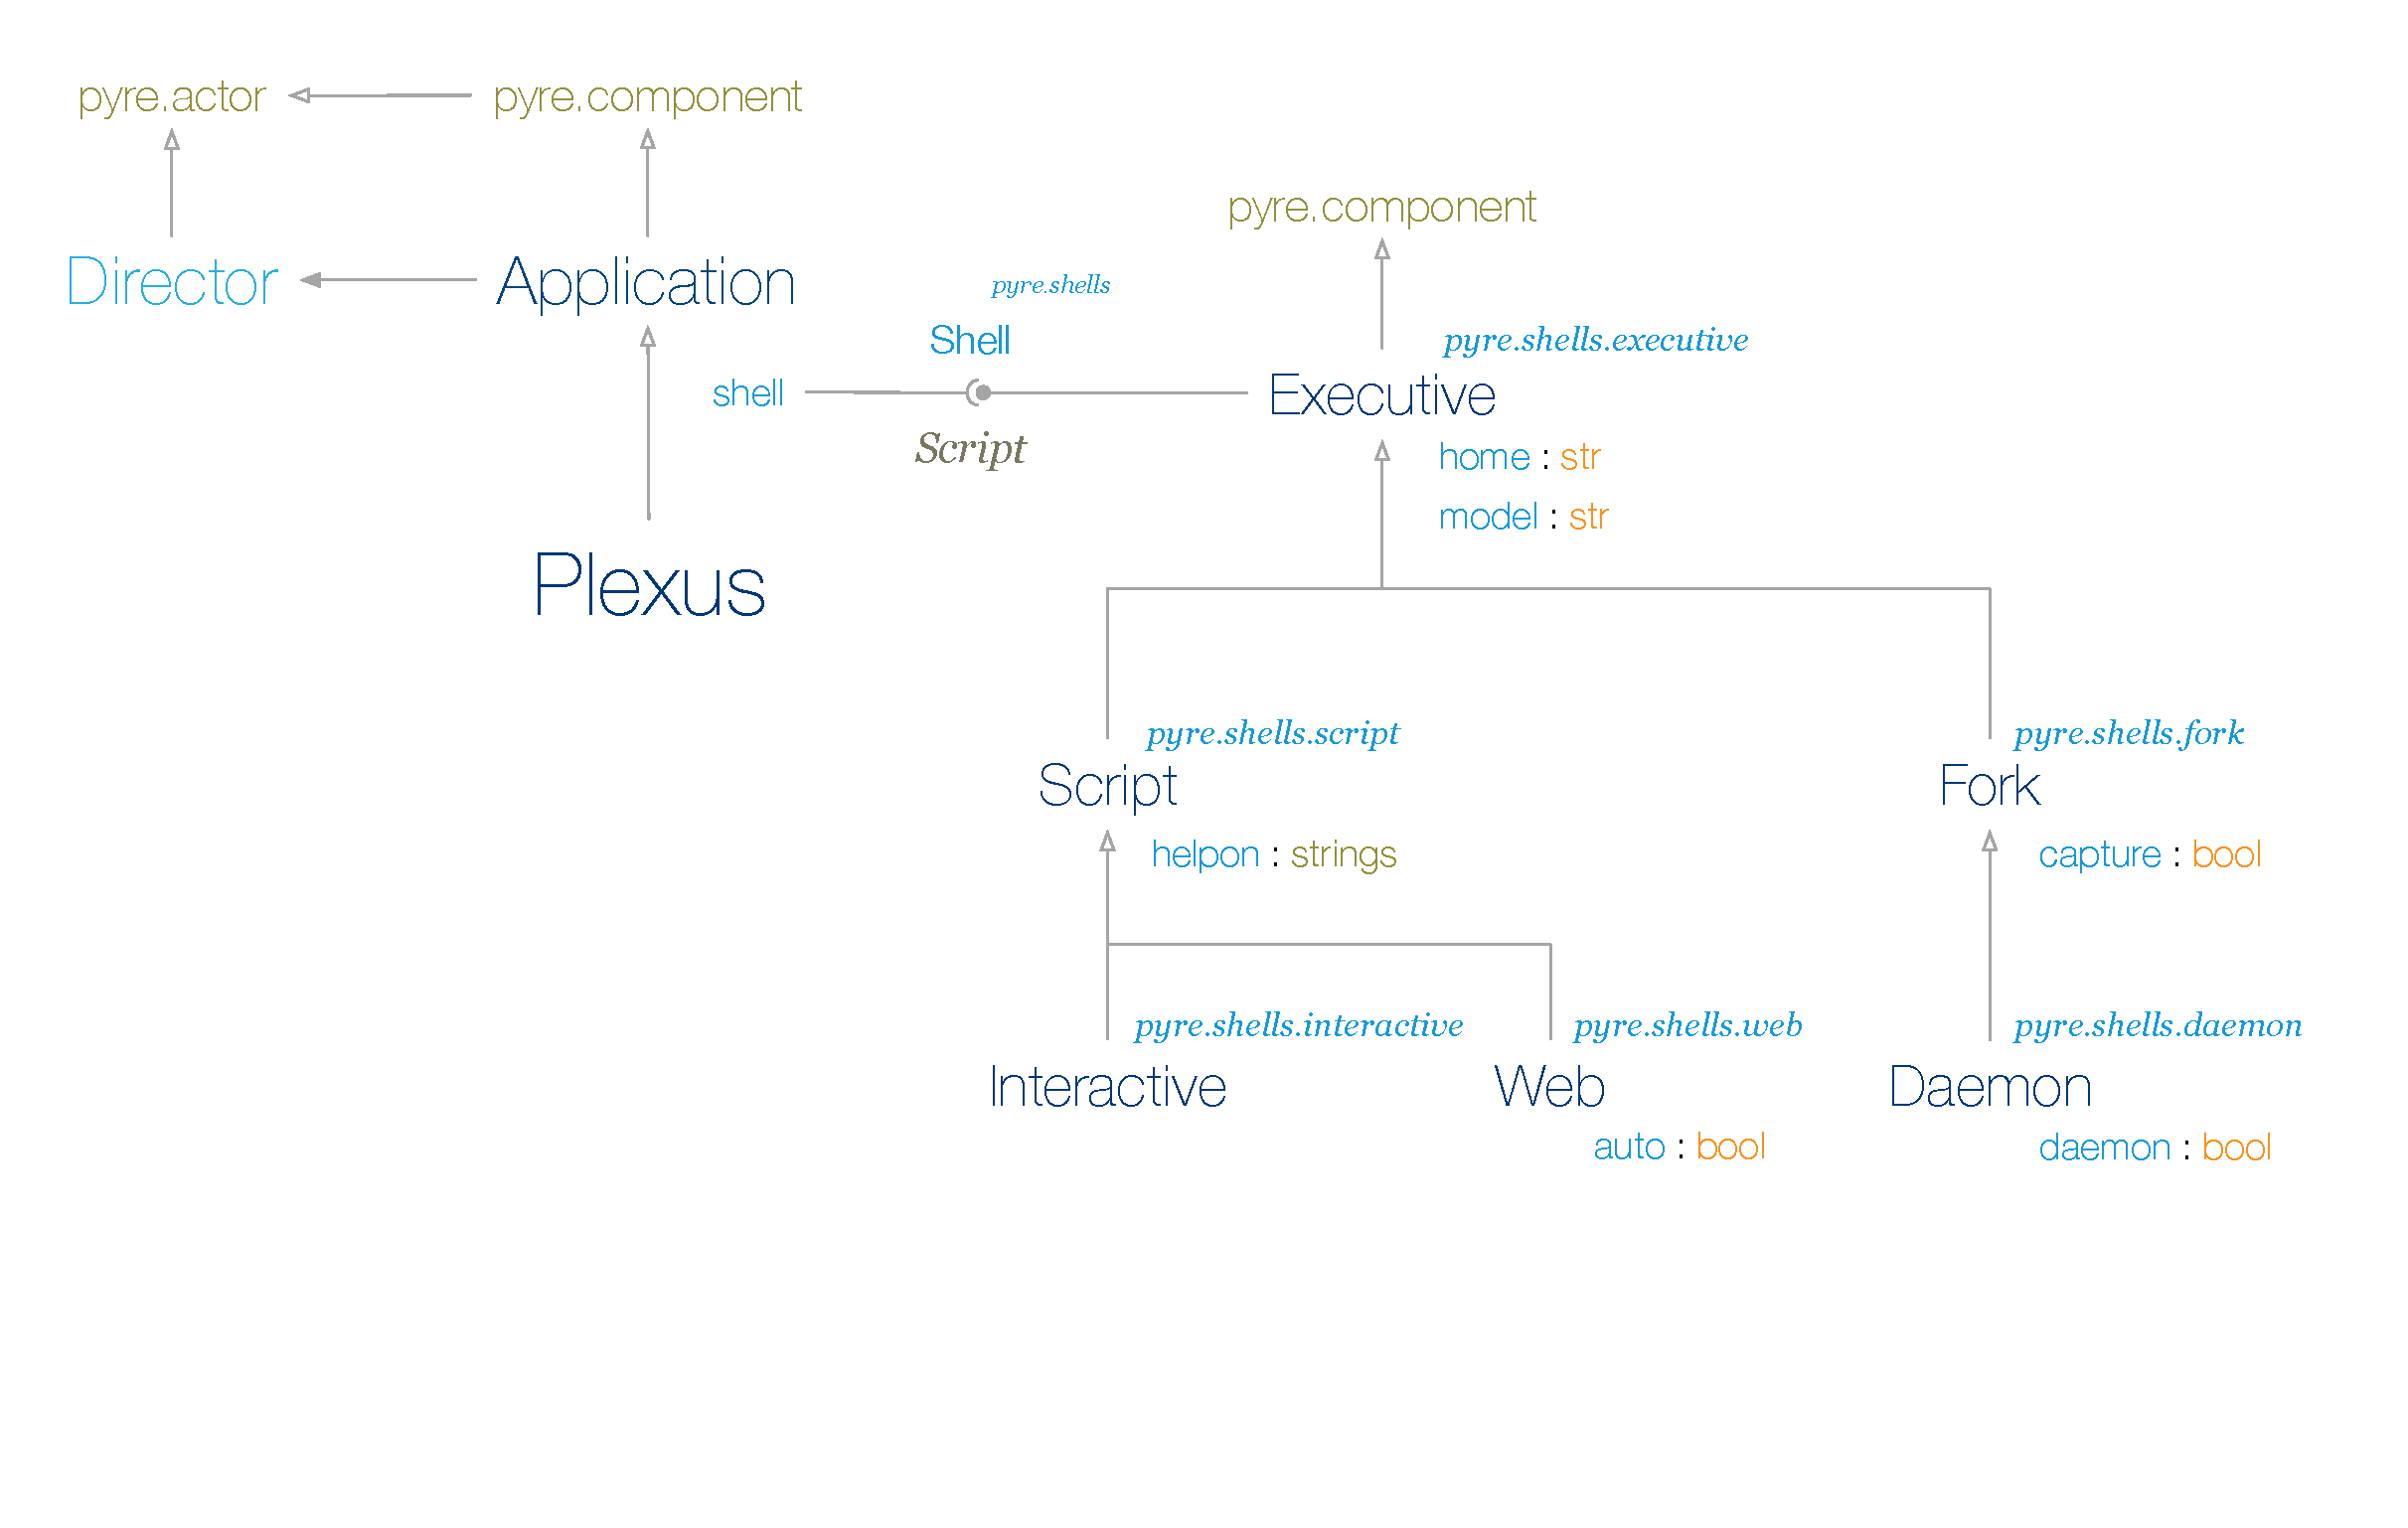
\includegraphics[width=0.9\textwidth]{pyre-plexus-shells}
    \end{center}
  }
  \only<6>{
    \begin{center}
      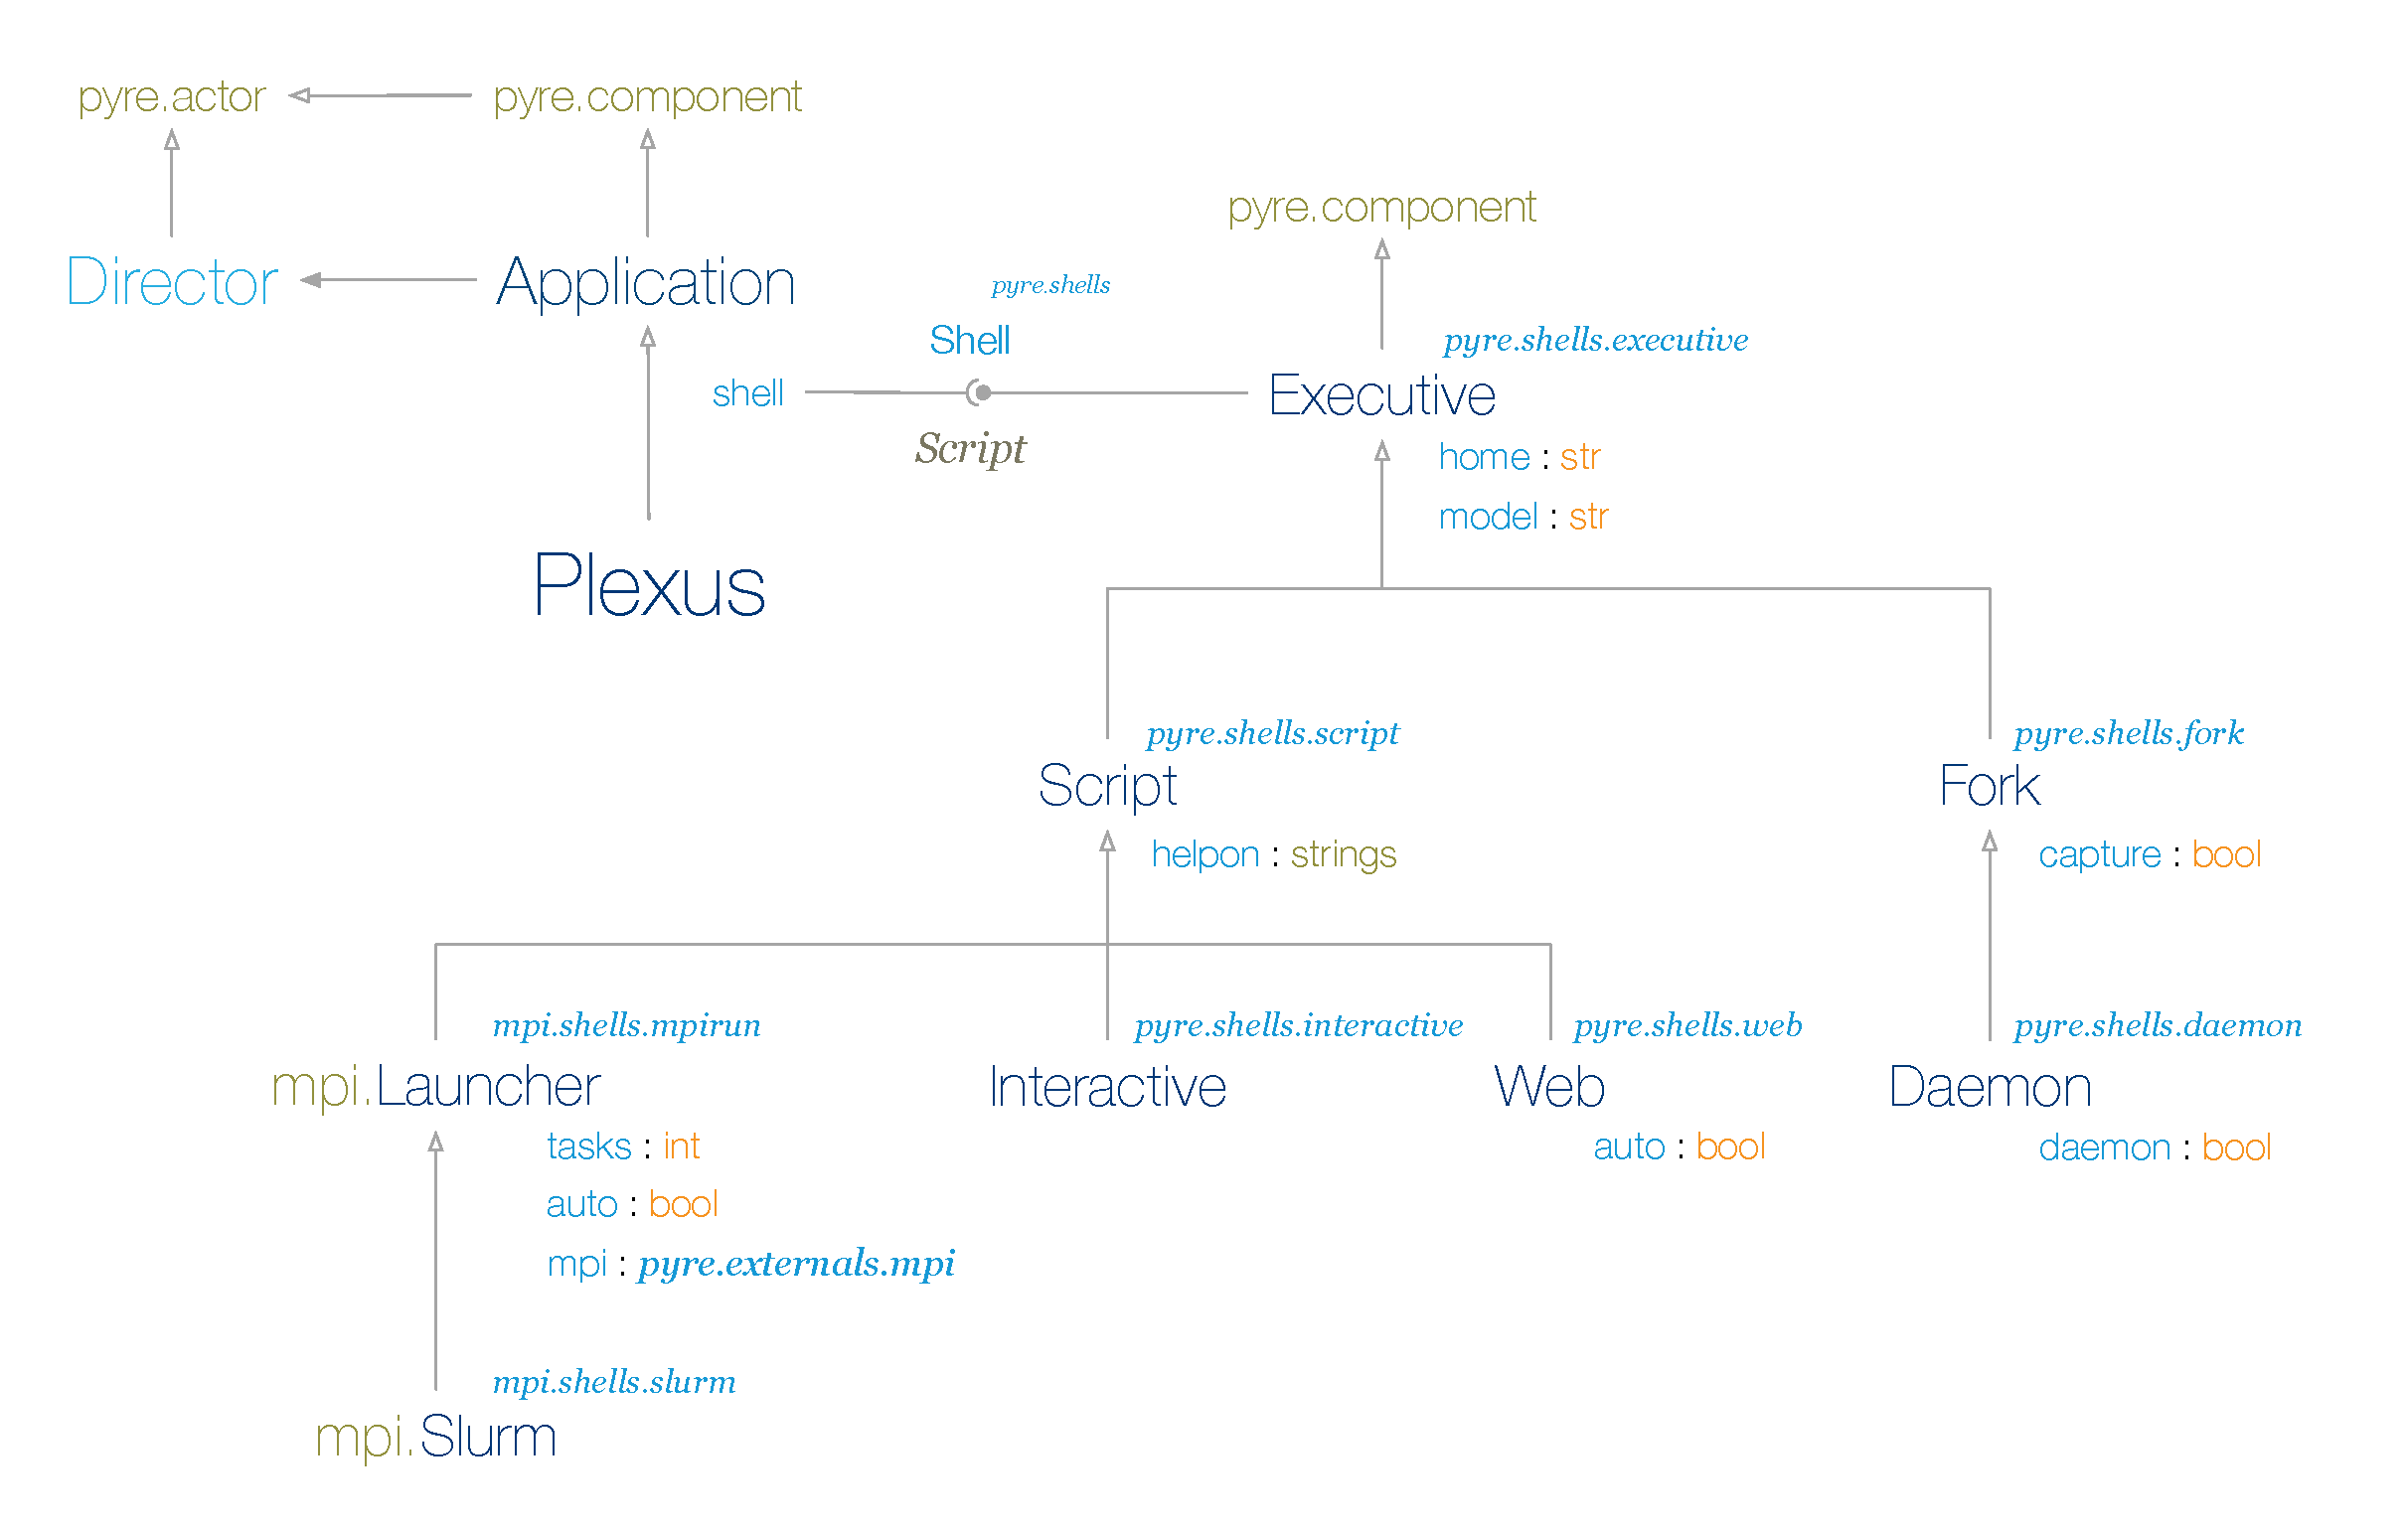
\includegraphics[width=0.9\textwidth]{pyre-plexus-mpi}
    \end{center}
  }
%
\end{frame}

% --------------------------------------

\TODO{
  \item configuration
    \begin{itemize}
    \item the full assignment uri
    \item assignments involving expressions and references
    \item wiring shortcuts for properly designed package namespaces
    \item having multiple configurations for the same property in the same file
    \item wiring a facility to a specific, perhaps pre\"existing component
    \item syntax rules for each format
    \end{itemize}
  \item explain plexus
  \item convert simple app into a plexus action
  \item private filesystems
  \item the standard filesystem layout
}


%%% Local Variables:
%%% mode: latex
%%% TeX-master: "../pyre"
%%% End:

% end of file
